\definecolor{LightCyan}{rgb}{0.88,1,1}
\newcolumntype{g}{>{\columncolor{LightCyan}}l}


\chapter{Conclusion}

Calculating average flux only depends on three variables. 
Although this calculation appears simple, estimating an average observational area can extremely difficult. 
Through establishing a versatile\comment{You've used this word before, but I think you need to better clarify what it means in this context?} method for calculating observable sky area, we can now estimate the D6 AllSky Camera's average flux and compare it to other systems.
As of this point, our data sample is too small to make any conclusive claims.  
As such, there are still steps that need to be taken to truly assess the feasibility of using the D6 AllSky Camera in fireball research.  
This section will detail some of our self-assessed points of critique as well as shed light on some possible future research directions.

\section{Results}
\inlinecomment{I'd really put this at the end of the data section. It feels very out of place here where everything else is more about critique and future directions.}
After attaining the number of events, total observation time, and average observational area, we found that the D6 AllSky Camera had an average flux of \hl{$->$}\SI{3.86E-7}{\per\hour\per\square\kilo\meter}\hl{$<-$}.
Table~\ref{table1} displays this value alongside the values that contributed to our flux calculation. 
As a point of comparison, Dr.~Jed Rembold measured an average flux rate of \SI{1.09E-7}{\per\hour\per\square\kilo\meter} when studying meteor impacts on the Moon. 
Clearly the Moon and Earth are inherently two different objects with different gravitational effects.
However they have similar locations within our solar system, and thus their average flux rates should share some resemblance.
The fact that the D6 AllSky Camera's fireball flux rate is of the same order of magnitude as research in the same field, we remain cautiously optimistic about the feasibility of our camera system.\comment{This sentence feel really choppy? Or is missing a word?}



\begin{table}[ht]
\setlength\extrarowheight{5pt}
\centering
\begin{tabular}{l|gg}
%\hline
&Value &Units \\
\hline
Number of Events & $6$ & events \\
%\hline
Average Area & $56,012.03$ & km$^2$ \\
%\hline
Total Time & $291.87$ & hr \\
\hline
Flux & $3.86 \times 10^{-7}$ & hr$^{-1}$km$^{-2}$ \\

%\hline
\end{tabular}
\caption{A display of our average flux rate alongside contributing variables.\inlinecomment{Use booktabs for all tables, and eliminate vertical rules. Also, if you are going to shade, I'd go light shades of gray only. Also, it seems like if you are going to make the comparison you did above to the lunar data, you should just bake the units into each entry in this table and include a column for the lunar values as a point of comparison.}}
\label{table1}
\end{table}

\section{Critique}

While there are a multitude of positives to take away from this research, there are many areas of improvement as well.  
The main critique of our work stems from a lack of sufficient data.
Flux estimates rely on a robust data sample, something that we were not able to attain this academic year. 
In the Fall of 2018, we also experienced some camera difficulties that led to data that was incompatible with our Photometry GUI software.\comment{I'm not sure these are camera difficulties or just being a different camera than what Photometry was tested predominantly with. That said, we are of course having extra noisy camera issues at the moment that could be acknowledged.}


\subsection{Data Size}

Throughout the history of fireball research, a sufficient data size has proven to be a vital characteristic of most notable findings.
In 1996, the Canadian camera network published a detailed analysis of the $259$ fireballs captured by their system \cite{halliday_innisfree_1981}.
Peter Brown, one of the most recognized figures in fireball research, released a paper in 2002 that detailed an analysis of $300$ fireballs as captured by the department of energy and defense\comment{Shouldn't that be capitalized?} \cite{brown_p_flux_2002}.
Surveys like these two have the luxury of calculating detailed flux estimates for fireballs with different energies or masses.\comment{Why do they and not us?}
By binning fireballs that share similar properties, these research groups can measure relationships between likelyhood of impact and fireball properties.
The value of average flux is often replaced then by the more detailed fireball energy distribution.
This makes comparing our system to existing systems slightly more difficult since net fireball flux rates are not always so widely reported.


Our system has captured a small fraction of the events found in the aforementioned research papers.\comment{Not the same events surely. And that is how this reads.}
Our lack of data isn't necessarily due to a lack of camera capability, and likely has to do with the total time observed. 
Observing a total of $34$ nights out of a possible $221$ yields a ratio of observing a little less than $16\%$ of nights. 
This low ratio is partially due to poor weather.
However, there were also nights where the camera was not placed outside due to scheduling complications.
\comment{Sentence about this becoming less of an issue as we finalize and become more confident with the camera software and leave it out in the field to observe for large tracts of time.}
Observing for more nights and capturing a larger number of fireball events will allow for more points of comparison to existing surveys.
This will in turn allow us to gain a stronger understanding of how our camera system compares to current professional systems.


\subsection{Camera Difficulties}

In the summer before the 2018-2019 academic calendar, the D6 AllSky Camera began having difficulty focusing on the night sky.\comment{It was later than this. The problem really only got super bad heading into this Spring.}
This led to images and videos containing lots of systematic noise.  
Figure~\ref{camera_noise} depicts the difference between an image with low and high noise.
Both images were taken with our same camera.
From these two images, it is clear that images and videos with high noise are more difficult to analyze.\comment{Reasons why?}
Coincidentally, the photometry program created by Luke Russell in 2017 and 2018 was created using test snapshots and videos taken without any noise issues.\comment{I don't think it is related to this. It was having issues tracking them even before the noise problems.}
The subsequent problem with noise led to an incompatibility with the photometry software.
Specifically, the part of the program that tracked the fireball location across frames was unable to do so when noisy pixels were found nearby the fireball.

\begin{figure}[ht!]
  \centering
  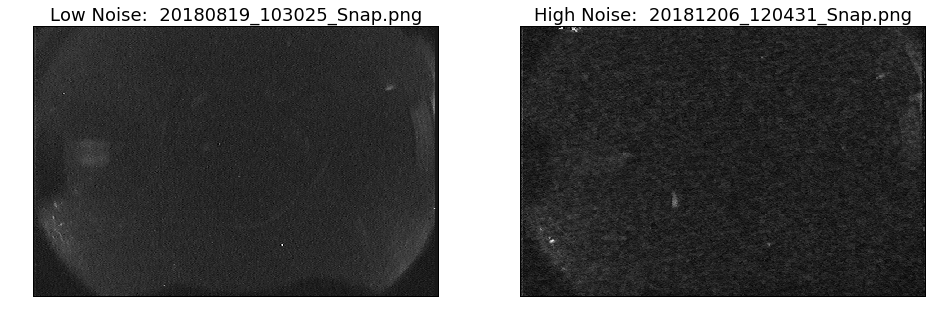
\includegraphics[scale=0.5]{images/low_and_high_noise.png}
  \caption{A D6 snapshot comparison of low and high noise. \inlinecomment{This caption is pathetic. :) Comment on it! Also, you should get your sizing such that the images do not extend beyond the text width.}}
  \label{camera_noise}
\end{figure}

Not only was the camera noise problematic for photometric analysis, but it also made star recognition more difficult.
In a majority of the snapshots captured by the D6 AllSky Camera, we were unable to recognize any celestial objects.\comment{A majority? How many are we talking? (That aren't also cloudy and so could have a chance at seeing something.}
A lower-noise level would allow us to recognize more stars which would add to our star catalog, and increase the number of data points used to determine observable area.
There is also a chance that we could detect dimmer stars with less-noisy data, leading to a stronger understanding of our camera's capabilities.

\section{Outlook}

Moving forward, the most important thing to focus on is data collection.
Once the problem with unusually high volumes of systematic noise is dealt with, we will have most of the framework established to create a running fireball catalog.
However, we will need to create a script that estimates a fireball's properties (energy, mass, size) given the photometry program's outputted light curve.
This project however should be fairly straightforward and will utilize the equations described in this paper's background chapter.\comment{Might as well reference them directly}

While a singular camera can serve an important role in fireball research, systems with multiple cameras stationed in different locations have certain benefits.
They allow for the triangulation of a given fireball which can then lead to more accurate velocity and position estimates.
With multiple systems, we could also estimate a fireball's orbital elements, and thus determine from whence it originated.
Next year, we hope to construct another D6 AllSky camera that will lead to more precise data collection. 
The prospect of a secondary system is exciting and will hopefully help prove that the D6 AllSky camera is a desirable alternative in fireball research.\comment{Technically, we'd like to show that D6 is up to the task \emph{before} investing in another system.}


\inlinecomment{You need to do a careful read through of your works cited and make sure they are rendering properly. Some seem to have empty fields that need fixing. For others it is not clear at all what sort of reference it even is. What is up with the one that just in the name of the camera?}
